\documentclass[a4paper,10pt]{article} % тип документа
% report, book

\usepackage[top=15mm,left=12.5mm, right=12.5mm]{geometry}
\usepackage[T2A]{fontenc}
\usepackage[utf8]{inputenc}
\usepackage[english,russian]{babel}
\usepackage{url}
\usepackage{ucs} % Для \textdegree


\usepackage{amssymb, amsmath, multicol, amsthm}
\usepackage{mathrsfs}
\usepackage{graphicx}
\graphicspath{{images1/}}
\usepackage{hyperref}
\usepackage{titleps} % Настраивает верхний колонтитул
\usepackage{icomma} % "Умная" запятая: $0,2$ --- число, $0, 2$ --- перечисление
%\usepackage{wrapfig} % Обтекание рисунков текстом - очень НЕ рекомендую, можно использовать окружение minipage
\usepackage{xifthen} 
\usepackage{xspace}
\usepackage{esvect} %красивый значок вектора
\usepackage{multirow} %Позволяет набрать задачу с дано и чертой справа от него
\usepackage{lipsum}
\usepackage{wrapfig}
\usepackage{floatrow} 
\usepackage{enumitem}
\usepackage{rotpages}

\usepackage[rgb,table,xcdraw]{xcolor}
\hypersetup{				% Гиперссылки
	unicode=true,           % русские буквы в раздела PDF
	colorlinks=true,       	% false: ссылки в рамках; true: цветные ссылки
	linkcolor=black,          % внутренние ссылки
	citecolor=black,        % на библиографию
	filecolor=magenta,      % на файлы
	urlcolor=blue           % на URL
}

\usepackage{tikz}
\usetikzlibrary{arrows,decorations.pathmorphing,backgrounds,positioning,fit,petri}

\binoppenalty=1000
\parindent=0pt
\headheight=10mm
\parskip=7pt
\textheight=178mm

\newpagestyle{main}{%
	\setheadrule{.4pt}%
	\sethead
	[\thepage][][\sectiontitle]
	{\subsectiontitle}{}{\thepage} }	
\pagestyle{main}

\let\leq\leqslant
\let\geq\geqslant

% Дублирует знаки математических операций при переносе на новую строку

\newcommand*{\hm}[1]{#1\nobreak\discretionary{}%
{\hbox{$\mathsurround=0pt #1$}}{}}

\usepackage[version=4]{mhchem}

% Нестандартные математические операторы

\newcommand{\divisible}{\mathop{\raisebox{-2pt}{\vdots}}}
\newcommand{\sgn}{\operatorname{sgn}}

% Сделать раздел/подраздел и добавить его в оглавление

\newcommand{\sect}[1]{\section*{#1}\sectionmark{#1}\addcontentsline{toc}{section}{#1}}
\newcommand{\subsect}[1]{\subsection*{#1}\subsectionmark{#1}\addcontentsline{toc}{subsection}{#1}}

\newcounter{prob}
\newcounter{example}

% команда \prob: Нумерация в стиле Задача 1.
% команда \complexprob: Нумерация для задач со звездочкой в стиле Задача 2*.
% команда \labeledprob: Нумерованная задача, на которую можно сослаться с помощью \refprob.

% Каждая из команд \prob, \complexprob и \labeledprob имеет необязательный аргумент, в котором указывается ссылка на источник задачи

\newcommand{\prob}[1][]{% 
\textbf{Задача \stepcounter{prob}\arabic{prob}% 
\ifthenelse{\equal{#1}{}}{}{\textsuperscript{\cite{#1}}}}.\xspace}

\newcommand{\example}[1][]{% 
\textbf{Упражнение \stepcounter{example}\arabic{example}% 
\ifthenelse{\equal{#1}{}}{}{\textsuperscript{\cite{#1}}}}.\xspace}

\newcommand{\complexprob}[1][]{% 
\textbf{Задача \stepcounter{prob}\arabic{prob}% 
\ifthenelse{\equal{#1}{}}{}{\textsuperscript{\cite{#1}}}}$^*$.\xspace}

\newcommand{\labeledprob}[2][]{%
\textbf{Задача \refstepcounter{prob}\label{#2}\arabic{prob}%
\ifthenelse{\equal{#1}{}}{}{\textsuperscript{\cite{#1}}}}.\xspace}

\newcommand{\refprob}[1]{\textbf{\ref{#1}}}

% Команды для оформления задач и решений

\newcommand{\sol}{\textit{Решение.} }
\newcommand{\ans}{\textit{Ответ:} }
\newcommand{\help}{\textit{Указание.} }

% Команды для оформления теории

\newcommand{\defin}{\textbf{Определение.} }
\newcommand{\theo}{\textbf{Теорема.} }
\newcommand{\note}{\textbf{Обозначение.} }
\newcommand{\ques}{\textbf{Вопрос.} }
\newcommand{\rem}{\textbf{Замечание.} }
\newcommand{\stat}{\textbf{Утверждение.} }
%\newcommand{\example}{\textbf{Упражнение.}  }	  

% Убрать квадратные скобки из списка источников
\makeatletter
\renewcommand{\@biblabel}[1]{\quad#1.}
\makeatother


%my preamble
% Рисунки
\usepackage{graphicx}
\usepackage{wrapfig}
\usepackage[font=small,labelfont=bf]{caption}

\usepackage{hyperref}
\usepackage[rgb]{xcolor}
\hypersetup{				% Гиперссылки
    colorlinks=true,       	% false: ссылки в рамках
	urlcolor=blue          % на URL
}

%  Русский язык

\usepackage[T2A]{fontenc}			% кодировка
\usepackage[utf8]{inputenc}			% кодировка исходного текста
\usepackage[english,russian]{babel}	% локализация и переносы


% Математика
\usepackage{amsmath,amsfonts,amssymb,amsthm,mathtools} 
\usepackage{systeme}

\usepackage{wasysym}


%Заговолок
\author{Команда менторов:)}
\title{Методичка к смене проета "Наука в Регионы"}
\date{\today}

%for inserting code
\usepackage{listings}
\usepackage{color}

\definecolor{dkgreen}{rgb}{0,0.6,0}
\definecolor{gray}{rgb}{0.5,0.5,0.5}
\definecolor{mauve}{rgb}{0.58,0,0.82}

\lstset{frame=tb,
  language=Java,
  aboveskip=3mm,
  belowskip=3mm,
  showstringspaces=false,
  columns=flexible,
  basicstyle={\small\ttfamily},
  numbers=none,
  numberstyle=\tiny\color{gray},
  keywordstyle=\color{blue},
  commentstyle=\color{dkgreen},
  stringstyle=\color{mauve},
  breaklines=true,
  breakatwhitespace=true,
  tabsize=3
}


\begin{document}

\begin{titlepage}

\begin{center}

\vspace*{-40pt}
\textsc{\large Федеральное государственное автономное образовательное учреждение высшего образования Московский физико-технический институт\\ (государственный университет)}\\
\vspace{48pt}


\includegraphics[width=0.6\textwidth]{images/logo.jpg}\\
\textsc{\Large Кафедра общей физики}\\[0.1cm] % Major heading such as course name
\textsc{\large Вопрос по выбору, 4 семестр}\\[0.5cm]

\vfill
{ \LARGE \textbf{ Генерация второй гармоники}}\\
\vspace{10pt}
{ \LARGE \textbf{в нелинейном кристалле}}\\
\vfill

{\large МФТИ}
{\large 2019}

\end{center}


\begin{minipage}{0.4\textwidth}
	\begin{flushleft} \large
		\textsf{Студенты}
		
		Ян \textsc{Логовский} \\[-0.15cm]
		
		Мария \textsc{Чикунова} \\[-0.15cm]

	\end{flushleft}
\end{minipage}
~
\begin{minipage}{0.4\textwidth}
	\begin{flushright} \large
		\textsf{Преподаватель}
		
		Владимир Владимирович\\[-0.15cm]
		\textsc{Усков} % Supervisor's Name
	\end{flushright}
\end{minipage}

\end{titlepage}



\newpage

\section{Теория}
Начнём с выявления причины появления второй гармоники. Для этого нам придётся рассмотреть электрон в решётке кристалла как линейный осциллятор. Он совершает вынужденные колебания под действием внешнего электрического поля E(t) светового излучения лазера и возвращающей силы F(x). Сразу отметим, что возникновение нелинейных эффектов может происходить только при величинах E(t), сравнимых с величиной внутриатомного поля E(t) $\sim 10^8 \div 10^9 \frac{V}{cm}$
\begin{equation}
m \ddot{x} = e E(t) + F(x)
\end{equation}

При больших x, решая (1), необходимо учитывать не только линейный по x член в разложении в  ряд Тейлора F(x), но и квадратичный. В таком случае решение будет иметь вид:
\begin{equation}
x(t) = \frac{\frac{e}{m} E_0}{{\omega_0}^2 - {\omega}^2} cos(\omega t) 
+ \frac{F''(0)}{4m {\omega_0}^2} \Big[\frac{\frac{e}{m} E_0}{{\omega_0}^2 - {\omega}^2}\Big]^2
+ \frac{F''(0)}{4m} \Big[\frac{\frac{e}{m} E_0}{{\omega_0}^2 - {\omega}^2}\Big]^2
\frac{cos2\omega t}{{\omega_0}^2 - (2 \omega)^2}
\end{equation}

Видим, что здесь появляется вторая мода колебаний с частотой $2 \omega$. А так как вторичные волны появляются как раз за счёт колебаний элетронов, то на выходе из нелинейного кристалла получаем свет с двумя длинами волн: $\lambda = \frac{2 \pi c}{\omega}$ и $\lambda / 2$.\\

Теперь нужно учесть то, что у кристалла есть какой-то размер, соответственно необходимо просуммировать вклады генерации вторичных волн с частотой $2 \omega$ от \textit{разных его частей}. Откуда получаем:
\begin{equation}
A^{(2 \omega)} \sim \frac{sin(k_0(\omega) \Delta n z)}{k_0(\omega) \Delta n z}
\end{equation}
Для наибольшей интенсивности излучения второй гармоники необходимо, чтобы $\Delta n = n(2 \omega) - n(\omega) = 0$. Но в области нормальной дисперсии - $\frac{dn}{d \omega} > 0$, откуда получаем $n(2 \omega) > n(\omega)$.
Однако мы всё-таки можем достичь того случая, когда $\Delta n =0$, воспользовавшись свойствами анизотропных кристаллов:
\begin{itemize}
\item в них волна расщепляется на обыкновенную с $n_0$ и необыкновенную с $n_e$
\item показатель преломления необыкновенной волны зависит от направления распространения, поэтому, построив сечение поверхности $n_e(\omega)$ в координатах направлений распространения волны в кристалле получим эллипс, а не окружность как в случае обыкновенной волны.
\item в отрицательных кристаллах $n_e - n_0 < 0$ в направлениях, отличных от оптической оси (ось, где распространяющийся луч не испытывет двойного лучепреломления - на рисунке ось Z).
\end{itemize}

При достаточной величине двулучепреломления $|n_e - n_0|$ возможно пересечиние эллипса $n_e(2 \omega)$ и сферы $n_0(\omega)$. Тогда в получившемся направлении $\theta_0$ с оптической осью для \textit{отрицательных} кристаллов получим:
\begin{equation}
n_0(\omega) = n_e(2 \omega)
\end{equation}
Угол $\theta_0$ называется углом синхронизма, именно в направлении $\theta_0$ с оптической осью можно наблюдать генерацию второй гармоники. Небольшое отклонение от данного направления ведёт к быстрому затуханию данной гармоники, что будет видно при исследовании зависимости $I_{2 \omega} (\Delta \theta)$.

\begin{center}
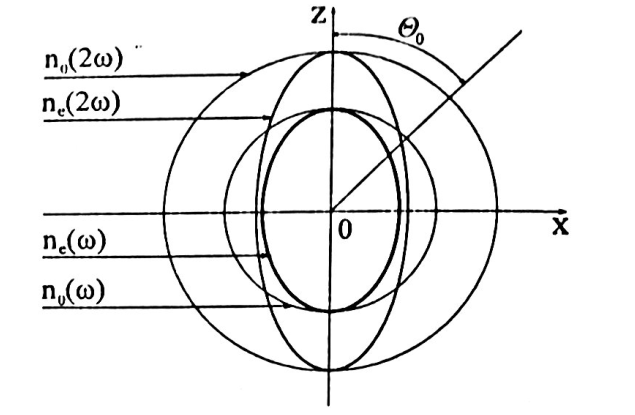
\includegraphics[width = 0.5\textwidth]{images/ellips}\\
\end{center}


\section{Установка}
\begin{center}
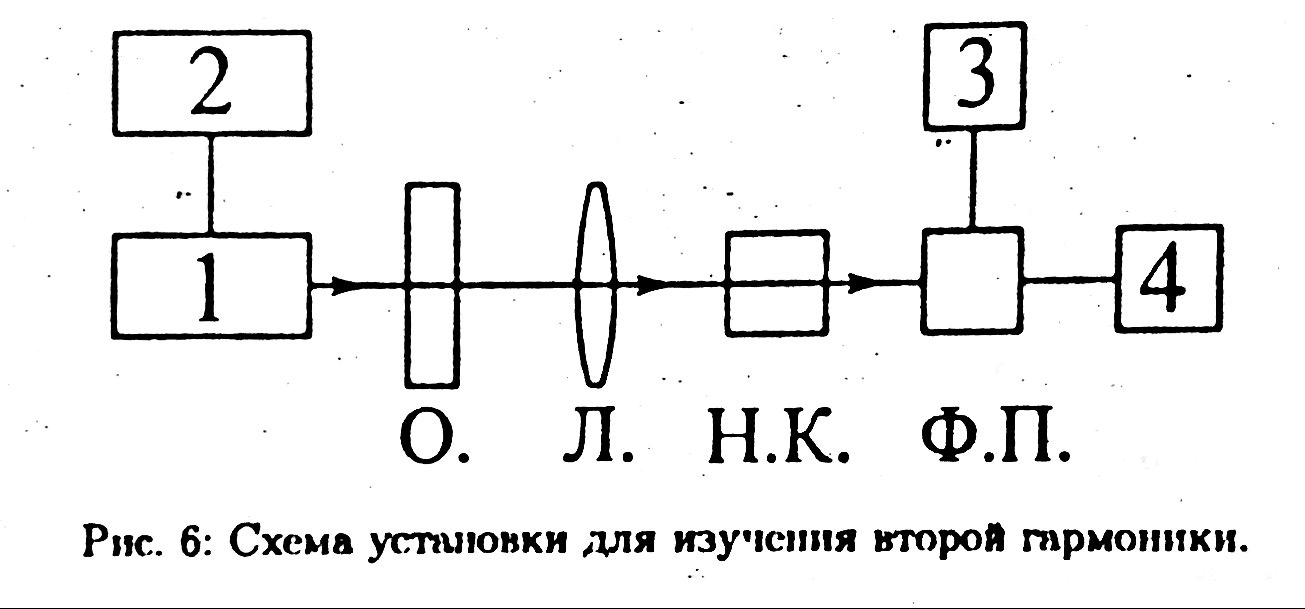
\includegraphics[width = 0.5 \textwidth]{images/setup.jpg}
\end{center}
Излучение лазера 1, пройля ослабитель О. и линзу-корректор Л., попадает в нелинейный кристалл Н.К., где его частота удваивается. Излучение удвоенной частоты далее попадает в фотоприёмник Ф.П. и регистрируется осциллографом 4.

\section{Интенсивность второй гармоники от интенсивности возбуждающей}
В данной таблице показаны значения интенсивности основной и второй гармоники от номера ослабителя, откуда можем построить зависимость $I_{2 \omega} (I_{\omega})$.\\
Как видно из формулы (1) - слагаемое с удвоенной частотой содержит амплитуду возбуждающей волны в квадрате. Следовательно, интенсивность излучения $I_{2 \omega}$ будет пропорциональна квадрату интенсивности $I_{\omega}$.
На графике интенсивности измерены в относительных величинах, однако качественно можно наблюдать, что наклон графика растёт, что соответствует квадратичной зависимости.

\begin{table}[H]
\begin{tabular}{|l|l|l|l|l|}
\hline
n     & 1   & 2   & 3   & 4   \\ \hline
$I_{\omega}$  & 4.4 & 3.6 & 3.2 & 2.6 \\ \hline
$I_{2 \omega}$ & 4.2 & 2.4 & 1.8 & 1.2 \\ \hline
\end{tabular}
\end{table}

\begin{center}
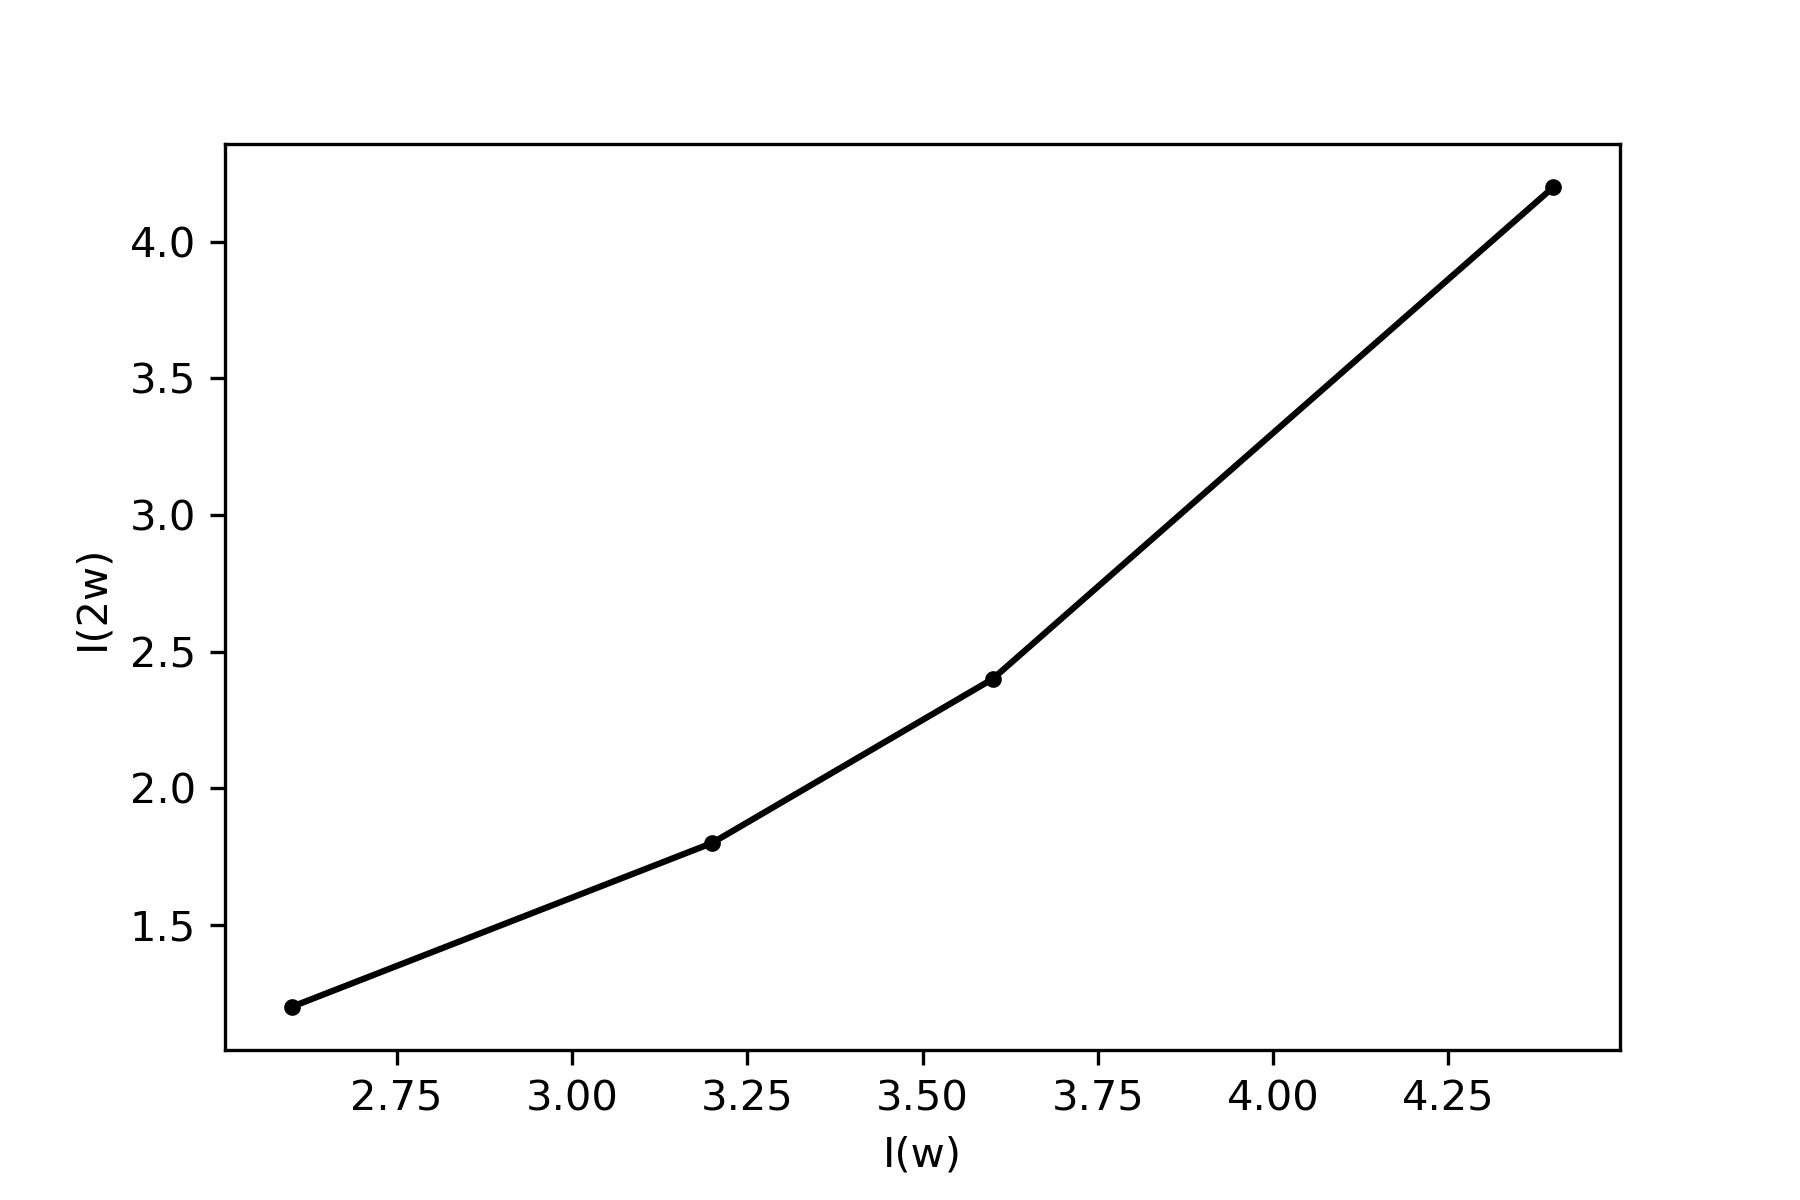
\includegraphics[width = 0.7\textwidth]{images/plot_1}
\end{center}

\section{Исследуем зависимость $I_{2\omega} (\Delta \theta)$}
При отклонениях от угла синхронизма $\theta_0$ интенсивность второй гамормоники быстро падает. Это вызвано большим влиянием расходимости световых пучков.

\begin{table}[H]
\begin{tabular}{|l|l|l|l|l|l|l|l|l|l|}
\hline
$\Delta \theta$, grad & 3’1’’ & 6’11’’ & 7’42’’ & 9’05’’ & 10’10’’ & 11’01’’ & 12’02’’ & 13’32’’ & 14’31’’ \\ \hline
$I_{2 \omega}$           & 4.2   & 3.6    & 3      & 2.4    & 1.6     & 1.2     & 0.8     & 0.4     & 0       \\ \hline
\end{tabular}
\end{table}

\begin{center}
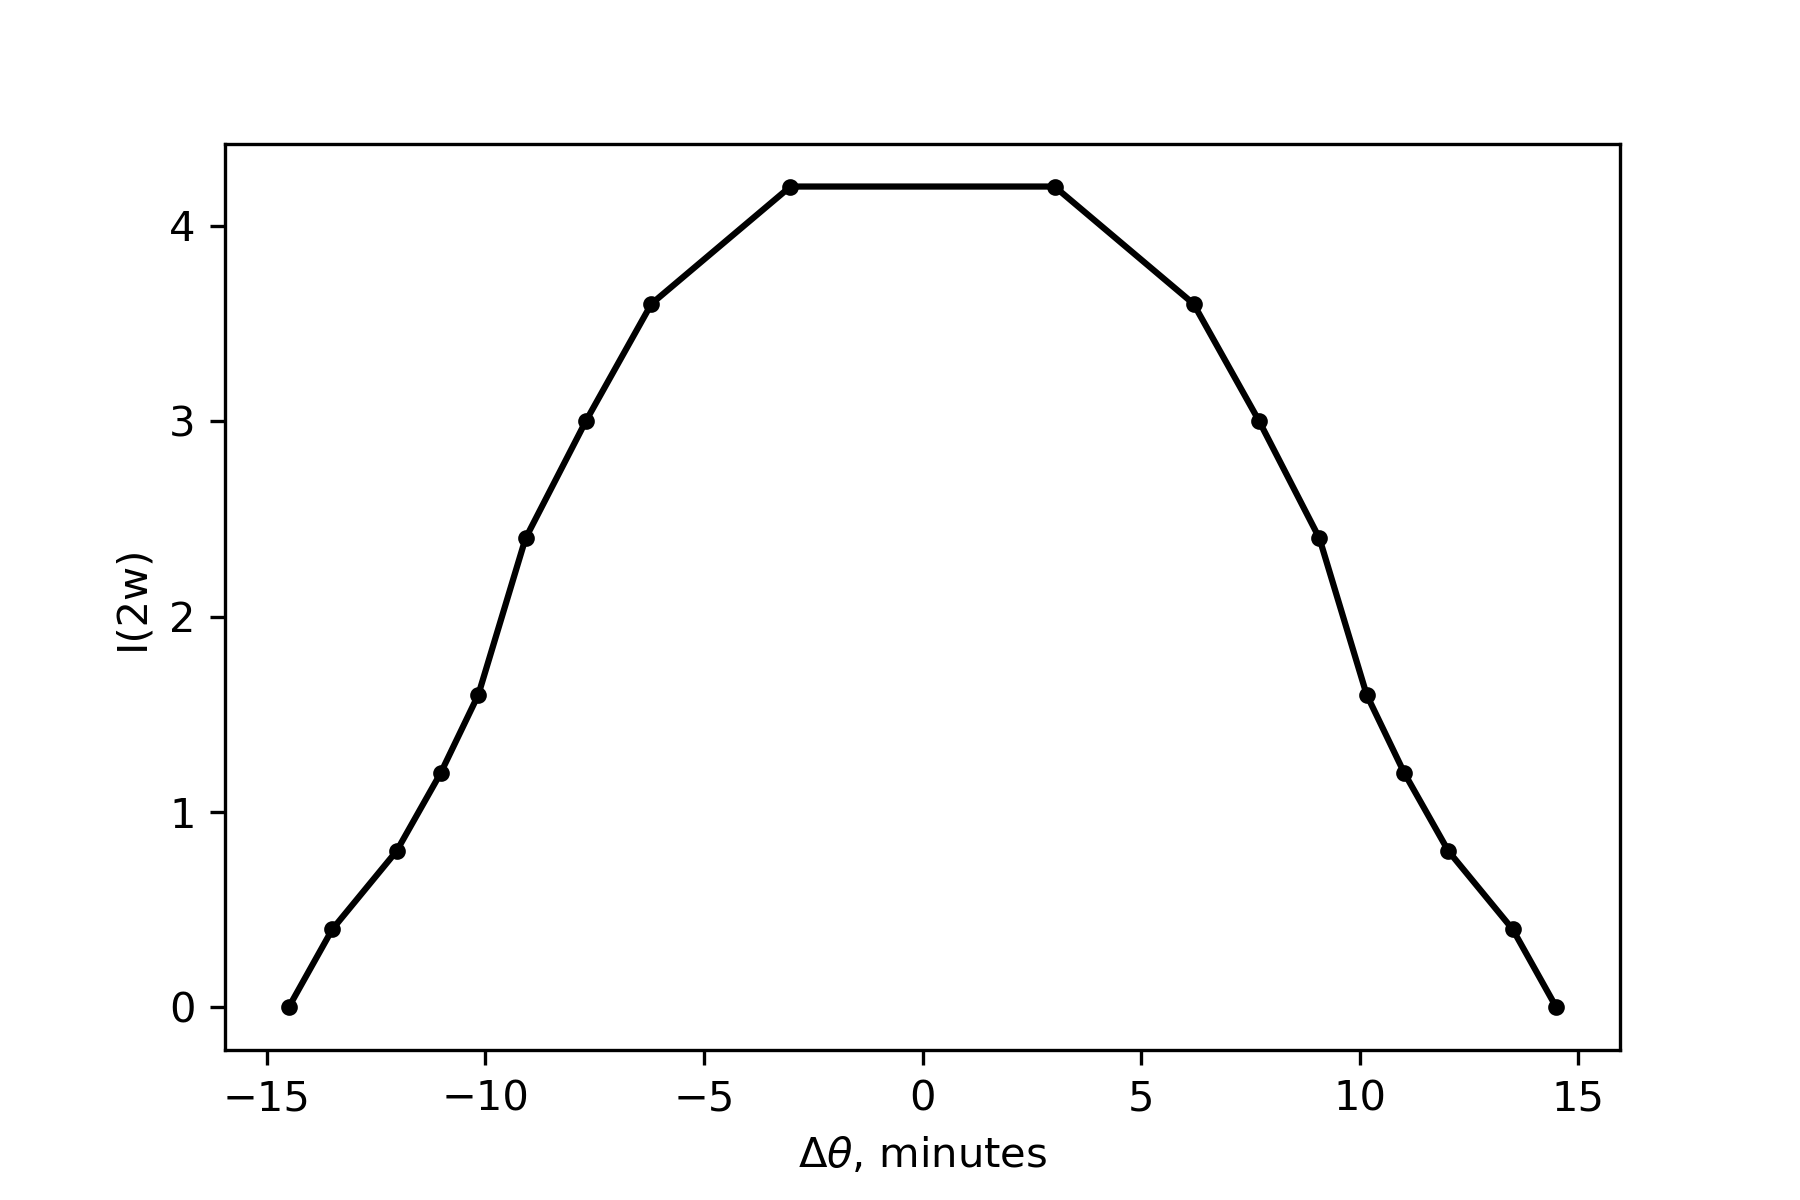
\includegraphics[width = 0.7\textwidth]{images/plot_2}
\end{center}

\section{Находим коэффициент преобразования}
Интенсивность света с двумя компонентами $I_{\omega + 2 \omega} = 7.8$\\
Интенсивность света без второй гармоники $I_{\omega} = 7.6$\\
Откуда коэффициент преобразования   $K = \frac{\Delta I}{I} = 0.0256 \approx 2,6 \%$\\\\
Малость коэффициента преобразования подтверждает, что энергия второй гармоники черпается из первичной волны, мощность которой уменьшается по мере углубления в среду.
Притом мощность волны с удвоенной частотой квадратично зависит от мощности первичной волны.
\section{Вывод}
Мы исследовали эффект генерации второй гармоники. Постановкой эксперимента убедились в наличии определённого направления в кристалле, в котором возможна генерация. Применили на практике способ преобразования инфракрасного излучения в видимое.


\end{document}